\section{VECTƠ TRONG KHÔNG GIAN}
\subsection{LÝ THUYẾT CẦN NHỚ}
\subsubsection{Tổng của hai véc tơ}
\begin{enumerate}[\iconMT]
	\item \indam{Định nghĩa:}
	\immini{Trong không gian, cho hai véctơ $\vec{a}$ và $\vec{b}$. Lấy ba điểm $O$, $A$, $B$ sao cho $\vec{OA}=\vec{a}$, $\vec{AB}=\vec{b}$. Ta gọi $\vec{OB}$ là \indamm{tổng của hai véctơ} $\vec{a}$ và $\vec{b}$, ký hiệu $\vec{a}+\vec{b}$.\\
		Phép lấy tổng của hai véctơ $\vec{a}$ và $\vec{b}$ được gọi là \indamm{phép cộng véctơ}.}
	{ \hspace{1cm}
	\begin{tikzpicture}[>=stealth,scale=.5,font=\footnotesize]
		\foreach \x\y\t in {3/0.4/A1,4./4.4/A2,9.5/4.3/B1,14.5/1.3/B2,5/0/O}
		\coordinate (\t) at (\x,\y);
		\coordinate (A) at ($(A2)-(A1)+(O)$);
		\coordinate (B) at ($(B2)-(B1)+(A)$);
		\foreach \a/\b in {A1/A2,B1/B2,O/A,A/B,O/B}
		{\draw[-{Stealth[length=2.5mm]}](\a)--(\b);}
		\node at ($(A1)!1/2!(A2)$)[left=-2pt]{$\vec{a}$};
		\node at ($(B1)!1/2!(B2)$)[above right=-2pt]{$\vec{b}$};
		\node at ($(O)!1/2!(A)$)[left=-2pt]{$\vec{a}$};
		\node at ($(A)!1/2!(B)$)[above right=-2pt]{$\vec{b}$};
		\node at ($(O)!1/2!(B)$)[rotate=7,above=-2pt]{$\vec{a}+\vec{b}$};
		\foreach \t/\g in {O/-140,A/90,B/0}
		\draw[fill=black] (\t)circle(1.2pt) +(\g:12pt)node{$\t$};
\end{tikzpicture}}
		\item \indam{Các quy tắc cần nhớ:} 
	\begin{itemize}
	\immini{\item [\ding{172}] Quy tắc ba điểm: Với ba điểm $A$, $B$, $C$, ta có
		\boxminit{$\vec{AB}  + \vec{BC}  = \vec{AC}$}
		\item [\ding{173}] Quy tắc hình bình hành: Cho $ABCD$ là hình bình hành, ta có
	\boxminit{$\vec{AB}  + \vec{AD}  = \vec{AC}$}}{
	\begin{tikzpicture}[scale=0.6, font=\footnotesize, line join=round, line cap=round]
		\begin{scope}
			\foreach \x\y\t in {0/0/A, -2/-2/B, 2.5/-1.5/C}
			\coordinate (\t) at (\x,\y);
			\foreach \a\b in {A/B, B/C,A/C}
			\draw[-{Stealth[length=2mm]}] (\a)--(\b);
			\foreach \t\g in {A/90, B/-100, C/-80}
			\draw[fill=black] (\t)circle(0.6pt) +(\g:8pt)node{$\t$};
		\end{scope}
		\begin{scope}[xshift=5cm]
			\foreach \x\y\t in {0/0/A, -1.5/-2/B, 2.5/-2/C,4/0/D}
			\coordinate (\t) at (\x,\y);
			\foreach \a\b in {A/B, A/D,A/C}
			\draw[-{Stealth[length=2mm]}] (\a)--(\b);
			\draw[dashed] (B)--(C)--(D);
			\foreach \t\g in {A/90, B/-90, C/-45,D/50}
			\draw[fill=black] (\t)circle(0.6pt) +(\g:8pt)node{$\t$};
		\end{scope}
\end{tikzpicture}}
		\immini{ \item [\ding{174}] Quy tắc hình hộp:
	Cho hình hộp $ABCD.A'B'C'D'$. Ta có
			\boxminit{$\vec{AB}  + \vec{AD}  + \vec{AA'}  = \vec{AC'}$}
			\begin{luuy}
				Hệ thức tương tự: \quad $\vec{BA}  + \vec{BC}  + \vec{BB'}  = \vec{BD'}$.
			\end{luuy}
		}{
			\begin{tikzpicture}[scale=0.6, font=\footnotesize, line join=round, line cap=round]
				\def\h{4}
				\foreach \x\y\t in {0/0/A',-1/-1.1/B',2.6/-1.1/C'}
				\coordinate (\t) at (\x,\y);
				\coordinate (D') at ($(A')+(C')-(B')$);
				\coordinate (A) at ($(A')+(0,2.5)$);
				\coordinate (B) at ($(B')+(0,2.5)$);
				\coordinate (C) at ($(C')+(0,2.5)$);
				\coordinate (D) at ($(D')+(0,2.5)$);
				\foreach \a\b in {A/B, A/D,A/C}
				\draw[-{Stealth[length=2mm]}] (\a)--(\b);
				\foreach \a\b in {A/A', A/C'}
				\draw[-{Stealth[length=2mm]},dashed] (\a)--(\b);
				\draw (D)--(C)--(B)--(B')--(C')--(D')--(D) (C')--(C);
				\draw[dashed](B')--(A')--(D');
				\foreach \t/\g in {A'/170,B'/-150,C'/-70,D'/0,A/100,B/170,C/-20,D/50}
				\draw[fill=black] (\t) circle(1pt)
				node[shift={(\g:7pt)}]{$\t$};
			\end{tikzpicture}
		} 
	\end{itemize}
	\item \indam{Tính chất:}
	\begin{gachsoc}
		\begin{itemize}
			\item[\ding{172}]Tính chất giao hoán: $\vec{a}+\vec{b}=\vec{b}+\vec{a}$;
			\item[\ding{173}] Tính chất kết hợp: $\left(\vec{a}+\vec{b}\right)+\vec{c}=\vec{a}+\left(\vec{b}+\vec{c}\right)$;
			\item[\ding{174}] Với mọi véctơ $\vec{a}$, ta luôn có: $\vec{a}+\vec{0}=\vec{0}+\vec{a}=\vec{a}$.
			\item[\ding{175}] Tổng của ba véctơ $\vec{a}$, $\vec{b}$, $\vec{c}$:\quad $\vec{a}+\vec{b}+\vec{c}=\left(\vec{a}+\vec{b}\right)+\vec{c}.$
		\end{itemize}
	\end{gachsoc}
\end{enumerate}
\subsubsection{Hiệu của hai véc tơ}
\begin{enumerate}[\iconMT]
	\item \indam{Véctơ đối:}
	\begin{itemize}
		\item [\ding{172}] Vectơ đối của $\vec{a}$ kí hiệu là $-\vec{a}$.
		\item [\ding{173}] Vectơ đối của $\vec{AB}$ là $\vec{BA}$, nghĩa là $-\vec{AB}=\vec{BA}$ (\textit{dùng để làm mất dấu trừ trước vectơ}).
		\item [\ding{174}] Vectơ $\vec{0}$ được coi là vectơ đối của chính nó.
	\end{itemize}
\vspace{-0.7cm}
\immini{
	\item \indam{Định nghĩa hiệu của hai véctơ:} Trong không gian, cho hai véctơ $\vec{a}$, $\vec{b}$. Ta gọi $\vec{a}+\left(-\vec{b}\right)$ là \indamm{hiệu của hai véctơ} $\vec{a}$ và $\vec{b}$, ký hiệu $\vec{a}-\vec{b}$.\\
	Phép lấy hiệu của hai véctơ được gọi là \indamm{phép trừ véctơ}.
	\item \indam{ Các quy tắc cần nhớ:}\\
	\begin{tcolorbox}[colframe=cyan,colback=red!3!white,boxrule=0.3mm]
		\begin{itemize}
			\item [\ding{172}] Với ba điểm $A$, $B$, $C$ ta có $\vec{AB}-\vec{AC}=\vec{CB}$.
			\item [\ding{173}] Hai véc tơ $\vec{a}$ và $\vec{b}$ đối nhau thì $\vec{a}+\vec{b}=\vec{0}$.
		\end{itemize}
	\end{tcolorbox}
}{\vspace{0.9cm}\hspace{1cm} 
\begin{tikzpicture}[scale=1, font=\footnotesize, line join=round, line cap=round]
	\foreach \x\y\t in {0/0/O,1.5/1/A,3.1/-0.4/B,-0.3/1/a1,1.1/1.6/b1}
	\coordinate (\t) at (\x,\y);
	\coordinate (a2) at ($(a1)+(A)$);
	\coordinate (b2) at ($(b1)+(B)$);
	\foreach \a\b in {a1/a2, b1/b2,O/A,O/B,B/A}
	\draw[-{Stealth[length=2mm]}] (\a)--(\b);
	\path (a1)--(a2)node[pos=0.5,above left]{$\vec{a}$}
	(b1)--(b2)node[pos=0.5,above]{$\vec{b}$}
	(O)--(A)node[pos=0.5,above left]{$\vec{a}$}
	(O)--(B)node[pos=0.5,below]{$\vec{b}$}
	(B)--(A)node[pos=0.7,right=3pt]{$\vec{a}-\vec{b}$};
	\foreach \t\g in {A/90, O/180, B/0}
	\draw[fill=black] (\t)circle(0.2pt) +(\g:5pt)node{$\t$};
\end{tikzpicture}}
\end{enumerate}
\subsubsection{Tích của một số với một véc-tơ}
\begin{enumerate}[\iconMT]
	\item \indam{Định nghĩa:} Cho số thực $k\ne 0$ và vectơ $\vec{a} \ne \vec{0}$. Tích của một số $k$ với vectơ $\vec{a}$ là một vectơ, kí hiệu là $k\vec{a}$, được xác định như sau:
	\begin{itemize}
		\item Cùng hướng với vectơ $\vec{a}$ nếu $k>0$, ngược hướng với vectơ $\vec{a}$ nếu $k<0$.
		\item Có độ dài bằng $|k| \cdot |\vec{a}|$.
	\end{itemize}
	\begin{luuy}
	$0\cdot \vec{a}=\vec{0}$ và $k\cdot \vec{0}=\vec{0}$.
	\end{luuy}
\immini{\indamm{ Ví dụ:} Theo hình vẽ bên, thì $\vec{b}=3\vec{a}$; $\vec{c}=-2\vec{a}$; $\vec{c}=-\dfrac{2}{3}\vec{b}$.
}{
	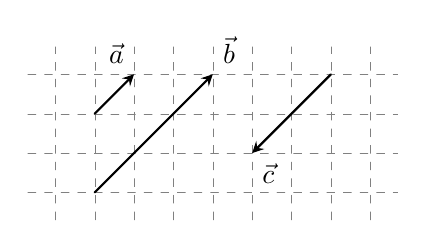
\begin{tikzpicture}[>=stealth,scale=0.5, line join=round, line cap=round]
		\draw[line width=0.05pt,gray,dashed] (-0.7,-0.7) grid (8.7,3.7);
		\draw[->,thick](1,2)--(2,3)node[above left]{$\vec{a}$};
		\draw[->,thick](1,0)--(4,3)node[above right]{$\vec{b}$};
		\draw[->,thick](7,3)--(5,1)node[below right]{$\vec{c}$};
\end{tikzpicture}}
	\item \indam{Hệ thức trung điểm, trọng tâm:}
	\immini{
	\begin{itemize}
		\item [\ding{172}] $I$ là trung điểm của đoạn thẳng $AB$ thì
		\begin{itemize}
			\item [$\bullet$] $\vec{IA}  + \vec{IB}  = \vec 0$;
			\item [$\bullet$] $\vec{IA}=-\vec{IB}$; $\vec{AI}=\dfrac{1}{2}\vec{AB}$;...
		\end{itemize}
		\item [\ding{173}] $G$ là trọng tâm của tam giác $ABC$ thì
		\begin{itemize}
			\item [$\bullet$] $\vec{GA}+\vec{GB}+\vec{GC}=\vec{0}$;
			\item [$\bullet$] $\vec{GA}=-\dfrac{2}{3}\vec{AK}$; $\vec{GA}=-2\vec{GK}$;...
		\end{itemize}
\end{itemize}}{
	\begin{tikzpicture}[scale=0.8, font=\footnotesize, line join=round, line cap=round]
		\begin{scope}
			\foreach \x\y\t in {-2/-2/A, 0/0/B}
			\coordinate (\t) at (\x,\y);
			\coordinate (I) at ($(A)!0.5!(B)$);
			\foreach \a\b in {A/B}
			\draw[] (\a)--(\b);
			\foreach \t\g in {A/-90, B/40,I/1200}
			\draw[fill=black] (\t)circle(0.6pt) +(\g:8pt)node{$\t$};
		\end{scope}
		\begin{scope}[xshift=4cm]
			\foreach \x\y\t in {0/0/A, -2/-2/B, 2.5/-2/C}
			\coordinate (\t) at (\x,\y);
			\coordinate (M) at ($(A)!0.5!(B)$);
			\coordinate (N) at ($(A)!0.5!(C)$);
			\coordinate (K) at ($(C)!0.5!(B)$);
			\coordinate (G) at ($(A)!2/3!(K)$);
			\foreach \a\b in {A/B, B/C, A/C, A/K, M/C, B/N}
			\draw[] (\a)--(\b);
			\foreach \t\g in {A/90, B/-100, C/-80, M/120, N/40, K/-90,G/60}
			\draw[fill=black] (\t)circle(0.8pt) +(\g:10pt)node{$\t$};
		\end{scope}
\end{tikzpicture}}
	\item \indam{Nhận xét:}
	\begin{itemize}
		\item[\ding{172}] Với hai véctơ $\vec{a}$ và $\vec{b}$ bất kỳ, với mọi số $h$ và $k$, ta luôn có
		\begin{enumerate}
			\item $k\left(\vec{a}+\vec{b}\right)=k\vec{a}+k\vec{b}$;
			\item $\left(h+k\right)\vec{a}=h\vec{a}+k\vec{a}$;
			\item $h\left(k\vec{a}\right)=\left(hk\right)\vec{a}$;
			\item $1\cdot \vec{a}=\vec{a}$;
			\item $\left(-1\right)\cdot\vec{a}=-\vec{a}$;
			\item $k\vec{a}=\vec{0} \Leftrightarrow \hoac{&\vec{a}=\vec{0}\\& k=0}$.
		\end{enumerate}
		\item[\ding{173}] Hai véctơ $\vec{a}$ và $\vec{b}$ ($\vec{b}$ khác $\vec{0}$) cùng phương khi và chỉ khi có số $k$ sao cho $\vec{a}=k\vec{b}$.
		\item[\ding{174}] Ba điểm phân biệt $A$, $B$, $C$ thẳng hàng khi và chỉ khi có số $k \neq 0$ để $\vec{AB}=k\vec{AC}$.
	\end{itemize}
\end{enumerate}
\subsubsection{Tích vô hướng của hai véc-tơ}
\begin{enumerate}[\iconMT]
	\item \indam{Góc giữa hai véctơ:}
	\immini{
			Trong không gian, cho $\vec{u}$ và $\vec{v}$ là hai véctơ khác $\vec{0}$. Lấy một điểm $A$ bất kỳ, gọi $B$ và $C$ là hai điểm sao cho $\vec{AB}=\vec{u}$, $\vec{AC}=\vec{v}$. Khi đó, ta gọi $\widehat{BAC}$ là góc giữa hai véctơ $\vec{u}$ và $\vec{v}$, ký hiệu $\left(\vec{u}, \vec{v}\right)$.
			\begin{luuy}
				$0^{\circ} \leq \left(\vec{u},\vec{v}\right) \leq 180^{\circ}$.
			\end{luuy}
			\begin{gachsoc}
				\begin{itemize}
					\item [$\bullet$] Nếu $\vec{u}$ cùng hướng với $\vec{v}$ thì $\left(\vec{u}, \vec{v}\right)=0^\circ$;
					\item [$\bullet$] Nếu $\vec{u}$ ngược hướng với $\vec{v}$ thì $\left(\vec{u}, \vec{v}\right)=180^\circ$;
					\item [$\bullet$] Nếu $\vec{u}$ vuông góc với $\vec{v}$ thì $\left(\vec{u}, \vec{v}\right)=90^\circ$.
				\end{itemize}
			\end{gachsoc}
}{\vspace{-0.5cm}
		\begin{tikzpicture}[scale=0.8, font=\footnotesize, line join=round, line cap=round]
			\foreach \x\y\t in {0/0/A,2/0.8/B,3.2/-1./C,-1/1/u1,-0.5/-1.5/v1}
			\coordinate (\t) at (\x,\y);
			\coordinate (u2) at ($(u1)+(B)$);
			\coordinate (v2) at ($(v1)+(C)$);
			\draw (-1.5,-1.2)--(3.5,-1.2)--(4.5,1)--(-0.5,1)--cycle;
			\draw[dashed] (A)--(u1) (B)--(u2) (A)--(v1) (C)--(v2);
			\foreach \a\b in {A/B, A/C,u1/u2,v1/v2}
			\draw[-{Stealth[length=2mm]}] (\a)--(\b);
			\foreach \t\g in {A/-170, B/0, C/50}
			\draw[fill=black] (\t)circle(0.6pt) +(\g:8pt)node{$\t$};
			\path (A) pic[draw,angle radius=9]{angle=C--A--B};
			\path 
			(u1)--(u2)node[pos=0.5,above]{$\vec{u}$}
			(v1)--(v2)node[pos=0.5,above]{$\vec{v}$};
	\end{tikzpicture}}
	\item \indam{Định nghĩa tích vô hướng của hai véc tơ:}
	Trong không gian, cho hai véctơ $\vec{u}$ và $\vec{v}$ khác $\vec{0}$.\\
	Tích vô hướng của hai véctơ $\vec{u}$ và $\vec{v}$ là một số, kí hiệu $\vec{u} \cdot \vec{v}$, được xác định bởi công thức
	\boxminit{$\vec{u} \cdot \vec{v}=|\vec{u}| \cdot |\vec{v}| \cdot \cos (\vec{u}, \vec{v})$}
	\vspace{-0.6cm}
	\begin{note}
		\begin{itemize}
			\item[\ding{172}] Trong trường hợp $\vec{u}=0$ hoặc $\vec{v}=0$, ta quy ước $\vec{u} \cdot \vec{v}=0$.
			\item[\ding{173}]  $\vec{u} \cdot \vec{u}=\vec{u}^2=|\vec{u}|^2$; \quad $\vec{u}^2 \geqslant 0$. $ \vec{u}^2 = 0 \Leftrightarrow \vec{u}=\vec{0}$.
			\item[\ding{174}]  Với hai véctơ $\vec{u}$, $\vec{v}$ khác $\vec{0}$, ta có $\cos (\vec{u},\vec{v}) = \dfrac{\vec{u} \cdot \vec{v}}{|\vec{u}| \cdot |\vec{v}|}$
			\item[\ding{175}]  Với hai véctơ $\vec{u}$, $\vec{v}$ khác $\vec{0}$, ta có $\vec{u} \perp \vec{v}  \Leftrightarrow \vec{u} \cdot \vec{v}= \vec{0}$.
		\end{itemize}
	\end{note}
	\item \indam{TÍnh chất:} Với ba véctơ $\vec{a}$, $\vec{b}$, $\vec{c}$ và số thực $k$, ta có:
	\begin{enumerate}[$\bullet$]
		\item $\vec{a}  \cdot \vec{b}= \vec{b} \cdot \vec{a}$;
		\item $\vec{a} \cdot \left( {\vec{b} + \vec{c}} \right) = \vec{a}  \cdot \vec{b} + \vec{a} \cdot \vec{c}$;
		\item $(k\vec{a}) \cdot \vec{b}= k(\vec{a}  \cdot \vec{b}) = \vec{a} \cdot (k\vec{b})$.
	\end{enumerate}
\end{enumerate}
